\section{Background}\label{sec:background}

%Give a short, self-contained summary of necessary
%background information. For example, assume you present an
%implementation of FFT algorithms. You could organize into DFT
%definition, FFTs considered, and cost analysis. The goal of the
%background section is to make the paper self-contained for an audience
%as large as possible. As in every section
%you start with a very brief overview of the section. Here it could be as follows: In this section 
%we formally define the discrete Fourier transform, introduce the algorithms we use
%and perform a cost analysis.
In this section we introduce the reader to Belief propagation and Top-N Recommendation.

\mypar{Belief Propagation}
Belief Propagation (BP) is a technique in the domain of machine learning to perform probabilistic inference on graphical models, out of which Bayesian Networks and Markov Random Fields are the most well known. The standard version of BP is designed to deal with factor graphs, a bipartite graph that can represent Bayesian Networks or Markov Random Fields. Nodes in a factor graph are either variables or factors. Variable-Nodes hold a belief about the variable assigned to them. A belief is a density function that assigns a probability to each state of the variable/node. Since the number of states of a variable is often finite this belief can be represented as a vector. Factor-Nodes, on the other hand, hold a belief about the joint probabilities of their neighbours. This, for example, means that if there are two Variable-Nodes connected to one Factor-Node the belief of the Factor-Node can be represented as a matrix, where entry $i,j$ holds the belief that one variable is in state $i$ while the other variable is in state $j$. Messages are send to inform neighbouring nodes about the beliefs of the sender. All receivers update their beliefs accordingly and then send updated messages to their neighbours. This is repeated until messages (and therefore beliefs) converge. Conceptually there are two types of messages, from Variable-Nodes to Factor-Nodes and from Factor-Nodes to Variable-Nodes. Understanding the concrete formulas is not required to follow this report but we give both update equations in figure \ref{eqn:bp_message} because they show nicely why this version of the belief propagation is often called the sum product algorithm. As you can see the update equations involve a product over all neighbouring nodes, followed by a sum that marginalizes over all variables excluding the one to which we want to send the message. This sum-product pattern will surface again when we describe our base line implementation in TODO:REF CODE IN SECTION 3.

\begin{figure}
\label{eqn:bp_message}
\begin{equation*}                                                            
\mu_{v\rightarrow a}(x_v) = \prod_{\hat a \in N(v)\backslash \{a\}} \mu_{\hat a\rightarrow v}(x_v)
\end{equation*}
\begin{equation*}                                                            
\mu_{a\rightarrow v}(x_v) = \sum_{x_a \sim x_v}f_a(x_a) \prod_{\hat v \in N(a)\backslash \{v\}} \mu_{\hat v\rightarrow a}(x_{\hat v})
\end{equation*}
\caption{Update equations for the BP algorithm. First for messages from variable node $v$ to factor $a$ and the second for messages from factor $a$ to variable node $v$; $x_v$ is the specific state for which we want to send our belief; $f_a(x_a)$ denotes the belief of the factor node $a$ about state $x_a$; $\mu$ is the message itself; $k \in N(i)\backslash j$ denotes all neighbours of $i$ except the neighbouring node $j$ and $x_a \sim x_v$ is used to denote all possible states that are consistent with state $x_v$.}
\end{figure}

The standard version of BP is designed to deal with acyclic graphs. The algorithm can, however, also be applied to graphical models containing loops, although convergence can no longer be guaranteed. In this context BP is often called \textit{Loopy Belief Propagation} (LBP). LBP problems are known for bad convergence and high computational costs. Nevertheless the approximated solution is often accurate enough to be used in real world applications. The illustrative work of Elidan et al. \cite{elidan2012residual} proposes a method to improve both convergence rate and, surprisingly, convergence (Elias TODO: convergence, not accuracy? Don't get it) by itself by propagating belief in an informed way through the graph. The technique is called \textit{Residual Belief Propagation} (RBP) for loopy graphs because a residual for each message is computed.
(Elias TODO: How is the residual computed? I want to write something like it reflects the importance of updating the message and we, therefore, should always update the message with the highest residual, but I'm not sure that is correct.)


\mypar{Top-N Recommendation}
Top-N Recommendation is the problem of generating a list of recommended items for a user $\hat u$. The list is based on the ratings of the user $\hat u$ as well as the ratings of the other users. Ha et al. \cite{Ha:2012:TRT:2396761.2398636} propose a method for Top-N Recommendation using loopy belief propagation. In this method the factor graph contains variable nodes for every users and every movies. The state of each node can either be\\
'1: $\hat u$ likes this user/movie' or\\
'2: $\hat u$ does not like this user/movie'. \\
Factors are used to connect movies with users. In more detail: we take all the ratings that are above average, meaning that a user $u_i$ really liked a movie $m_j$. We then create a factor connecting $u_i$ with $m_j$. This factor will have four states (2x2 matrix). We set the values $(1,1)$ and $(2,2)$ to $0.5 + \alpha$, $alpha = 0.0001$ to denote our belief that if user $\hat u$ likes either the movie $m_j$ or the user $u_i$, he will probably like the other one as well (transitivity of 'like'). Furthermore we set $(1,2)$ and $(2,1)$ to $0.5 - \alpha$ to express our belief that it is unlikely that user $\hat u$ only likes the movie or the user but not both.
Furthermore we already know a few movies that $\hat u$ likes/dislikes. This means for every rating from $\hat u$ for movie $m_j$ we set the belief of node $m_j$ to reflect that rating. In our concrete example ratings could vary between 1 and 5 stars which meant we would map a rating of 5 to $[0.9,0.1]$, a rating of 4 to $[0.7,0.3]$, 3 to $[0.5,0.5]$, 2 to $[0.3,0.7]$ and 1 to $[0.1,0.9]$. All other beliefs are initialized with $[0.5,0.5]$.

Figure \ref{top_n_graph} shows a small factor graph for  $\hat u = u_2$ where user $u_1$ has rated the movies $m1,m2$, $u_2$ the movie $m_2$ and $u_3$ the movies $m_1,m_2$ and $m_3$. Initially it is only known, that user $u_2$ likes the movie $m_2$ with a probability of 0.7. 
Using loopy belief propagation the most important messages are sent through the factors and the belief is propagated from observed nodes to unobserved nodes (see Figure \ref{top_n_graph_important_msg}). When the belief propagation converges each movie has a probability "User $\hat u$ likes movie $j$". Figure \ref{top_n_graph_final_state} shows a possible final state. The movies can be sorted by these probabilities and the top N elements are returned. In this example movie $m_1$ would be the top-one recommendation for user $u_2$.

% TODO why u no horizontal display?
\begin{figure}[h]\centering

%\subfloat{
    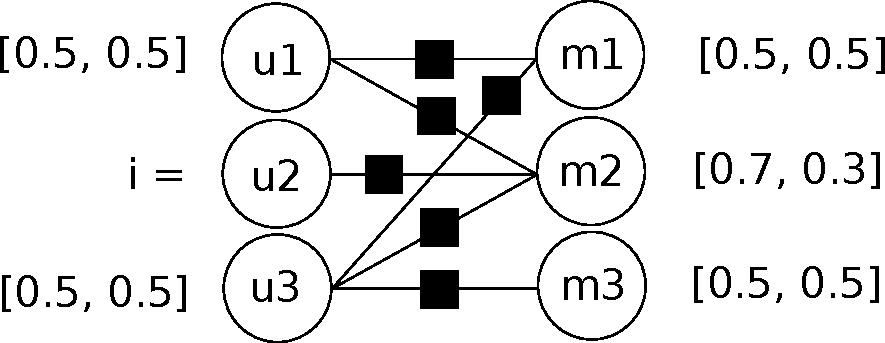
\includegraphics[scale=0.33]{graphics/top-n-graph.pdf}
\caption{Factor Graph for predicting top-n movies for user $u_2$. The dark squares are the factors. The values in [] show the probabilities for the random variables being in state "like" or "don't like".\label{top_n_graph}}
 %}

%\subfloat{
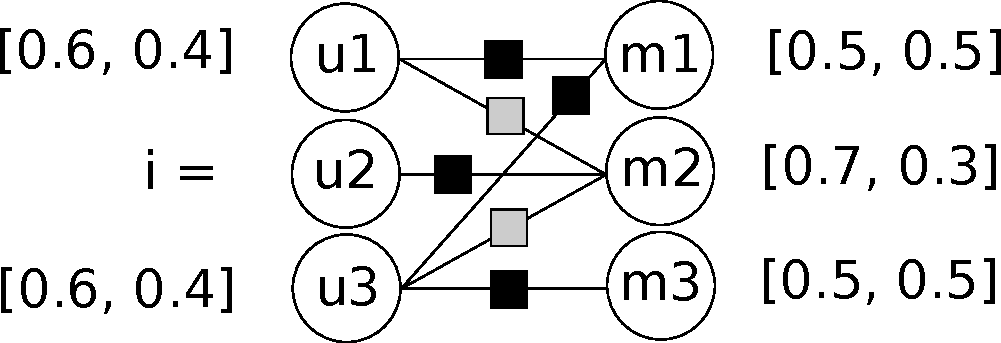
\includegraphics[scale=0.33]{graphics/top-n-important-messages.pdf}
  \caption{Belief is propagated from observed node $m_2$ to unobserved notes \label{top_n_graph_important_msg}}
  %} 

    %\subfloat{
    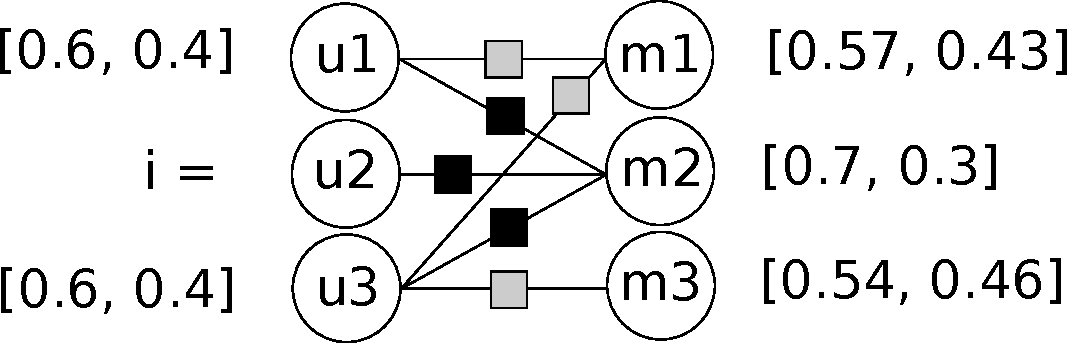
\includegraphics[scale=0.33]{graphics/top-n-final.pdf}
  \caption{A possible final state for top-n recommendation. Movie $m_1$ is the top recommendation for user $u_2$. \label{top_n_graph_final_state}}
%  }

\end{figure}

\mypar{Cost Analysis}

\textbf{TODO}

%\mypar{Discrete Fourier Transform}
%Precisely define the transform so I understand it even if I have never
%seen it before.
%
%\mypar{Fast Fourier Transforms}
%Explain the algorithm you use.
%
%\mypar{Cost Analysis}
%First define you cost measure (what you count) and then compute the
%cost. Ideally precisely, at least asymptotically. In the latter case you will need to instrument your code to count
%the operations so you can create a performance plot.
%
%Also state what is
%known about the complexity (asymptotic usually) 
%about your problem (including citations).